% The manuscript for P1EDA, short paper. 

\documentclass[11pt,letterpaper]{article}
\usepackage{naaclhlt2015}
\usepackage{times}
\usepackage{latexsym}
\usepackage{microtype}
\usepackage{amsmath,amssymb}
%\usepackage{microtype}
\usepackage{graphicx}
\usepackage{rotating}
\setlength\titlebox{6.5cm}    % Expanding the titlebox

\title{Multi-Level Alignments As an Abstraction Layer for Extendable,
  Multilingual Textual Entailment}


% \author{Author 1\\
% 	    XYZ Company\\
% 	    111 Anywhere Street\\
% 	    Mytown, NY 10000, USA\\
% 	    {\tt author1@xyz.org}
% 	  \And
% 	Author 2\\
%   	ABC University\\
%   	900 Main Street\\
%   	Ourcity, PQ, Canada A1A 1T2\\
%   {\tt author2@abc.ca}}

\date{}

\begin{document}
\maketitle
\begin{abstract}
  Textual Entailment technology has become more robust over the last
  years. Nevertheless, state-of-the-art models still rely on
  hand-crafted, incompatible data structures, which makes exchange of
  components very difficult in practice. In this paper, we introduce
  {\em multi-level alignments} as a very general representation to
  store information relevant for deciding entailment that can store
  many kinds of information. 
%, can be translated easily into features,
%  and is applicable across languages. 
  We demonstrate that a very simple open-source, pilot implementation
  of the approach already competes with much more complex
  state-of-the-art open-source TE engines across three languages. 
\end{abstract}

\section{Introduction}
A key challenge of Natural Language Processing is to determine what
conclusions can be drawn from a natural language text, a task known as
\textit{Textual Entailment} (TE, Dagan and Glickman
2004).\nocite{dagan04:_probab_textual_entail} The ability to recognize
TE helps dealing with surface variability in tasks like Question
Answering~\cite{harabagiu-hickl:2006:COLACL}, Intelligent Tutoring
\cite{nielsen09:_recog_entail_in_intel_tutor_system}, or Text
Exploration \cite{berant2012learning}.

TE technology has matured substantially over the last decade. Numerous
engines have been developed that implement a wide range of algorithms
and make use of many types of linguistic knowledge resources. It is
now much easier for end users to utilize TE engines. Recent progress
in the development of a common architecture for TE even makes it
possible to exchange various modules (such as resources,
pre-processing pipelines) fairly easily \cite{EOP-arch}.

%However, developers and researchers are still out of luck: 
However, improving an existing TE engine is still a very hard task:
The core TE algorithms themselves are generally not designed to be
extendable or interoperable. Therefore, unlike pre-processing modules 
or knowledge resources, changes to the core algorithms (like adding
support for a new language or a new aspect of analysis) are often very
hard, if not impossible. This often forces the next generation of TE
researchers to write their own core algorithms again from scratch. 

In this paper, we address this problem by proposing an approach to TE
that revolves around a central representation layer called {\em
  multi-level alignment} which can encode many relevant phenomena for
entailment. The use of multi-level alignments encourages the modular,
extensible development of TE algorithms that separate neatly into
``alignment producers'' and ``alignment consumers''. This makes it
easier to future researchers and developers to change analysis
components or add new ones. 
%\marginpar{SP: that's just a claim, right?}
%Gil: I agree. ``producer'' ``consumer'' sounds also clear. 

We also demonstrate our pilot implementation of this approach and
show evaluation results for English, German and Italian. It utilizes
only a minimal number of analysers, coupled with a set of basic
language-independent features, and thus can be regarded as a baseline
of the performance achievable with this approach.  The results are
surprisingly good and already compete with the best open-source
engines available for each target language.

\section{TE with Multi-Level Alignments}

The quality of the word alignment between a Text (T) and a Hypothesis
(H) has been used very early as a feature to decide TE. When research
showed that alignment strength on its own can be misleading
\cite{maccartney-EtAl:2006:HLT-NAACL06-Main}, alignment was 
understood as an intermediate step whose outcome is a set of
correspondences between parts of T and H that can be used to define
(mis-)match features. Alignments can be established at the
word level, phrase level \cite{MacCartney:EMNLP08}, or dependency
level \cite{dinu-wang:2009:EACL}. Dagan et
al. \shortcite{RTE-book} generalized various TE algorithms into
universal alignment-based approach with six steps: pre-processing,
enrichment, candidate alignment generation, alignment selection, and
classification. 

\paragraph{Proposal.} Our proposal is similar to, but simpler than,
Dagan et al.'s. Figure \ref{fig:1} shows the data flow.

\begin{figure}[t!b]
  \centering
  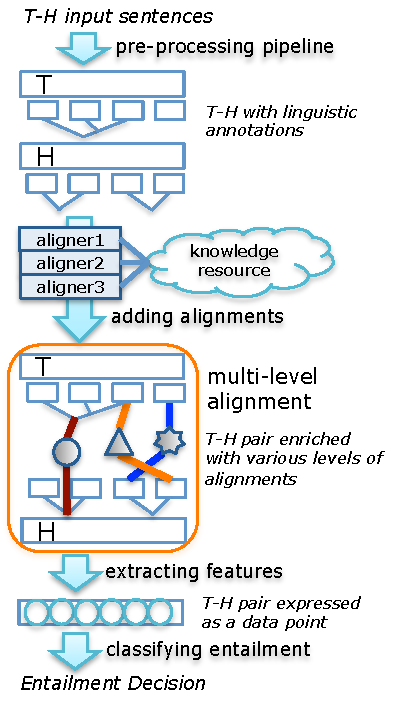
\includegraphics[width=0.9\columnwidth]{figures/figure1.pdf}
  \caption{Dataflow of the proposed approach}
  \label{fig:1}
\end{figure}

First, Text and Hypothesis are linguistically pre-processed. Then, the
annotated T-H pair becomes the input for various independent aligners,
which have access to knowledge resources and can compute any evidence
for or against entailment that can be represented as a weighted
alignment between any linguistic levels of H and T. Note that this
includes many analyses not normally treated as alignment, e.g. match
or mismatches in negation or modality between parts of T and H, or the
location of inference rules. The union of all alignments forms the
central data structure, the {\em Multi-Level Alignments}.

The next step is feature extraction. Features can be extracted on the
basis of individal alignments, or from sets of alignments. We assume
that the features form a vector describing the T-H pair, and that the
last step is supervised entailment classification.

\paragraph{Discussion.} The main difference to Dagan et al.'s proposal
is that we intentionally leave out the step of {\em alignment
  selection} which explicitly selects a single alignment for each part
of H or T, typically the globally most probable one. Our decision to
forgo selection is grounded in our design of Multi-Level Alignments as
a repository that supports coexistence of information from different
sources. This has the following benefits: (a) aligners become
decoupled in that adding a new aligner does not have a direct impact
on the global outcome; (b) alignments produced by different aligners
can have different semantics, e.g. positive (match) or negative
(mismatch); (c) interactions between alignments can still be captured
by defining features in the feature extraction step.

In this manner, Multi-Level Alignments serves as an abstraction layer
that encourages the development of small, self-contained modules that
contribute to TE recognition. Each of these modules consists of two
parts: an aligner, and a set of feature extractors. A priori, each
module can be defined independently; to introduce interactions with
other modules, it should be sufficient to extend the feature
extractors.

The practical benefit for the developer is that even relatively
complex TE systems use a small set of well-defined interfaces, which
makes the whole algorithm easy to manage, even on the implementation
level. The startup cost is getting acquained with the common data
structure of Multi-Level Alignments. We believe that developers are
willing to pay this cost, especially when this provides them with a
platform that supports multilingual preprocessing.

\section{Implementation and Evaluation}
\label{sec:impl}

We describe a pilot implementation of the approach and two evaluation
results in three languages (EN, DE, IT). The system is available
online.\footnote{{URL} anonymized.} 

%Multi-Level Alignment
%approach to test its potential by evaluating it on two use cases in
%three languages (DE, EN, IT). 

\subsection{Technical Foundations.}  
\label{sec:techn-found}

We implement the Multi-Level Alignment approach within an open source
TE development platform \cite{EOP-arch}. The platform provides various
multilingual pre-processing pipelines and knowledge resources such as
WordNet, VerbOcean, etc., under a shared API. For pre-processing, we
use TreeTagger-based pipelines for all three languages.

Another important service that is provided by the platform is the
ability of storing a wide range of linguistic annotations in a common,
language-independent data representation. The platform uses UIMA CAS
\cite{d04:_uima} as the data container, adopts the DKPro type system
\cite{DKpro}, and defines annotation types which can be extended in a
controlled manner. We used this capability to introduce a multilingual
Multi-Level Alignment layer %(links with types, labels and weights)
with relatively little implementation effort.
%By
%utilizing those existing modules of a common platform, we were able to
%concentrate on the core-algorithm implementations.

\subsection{A Minimal Set of Aligners}

The pilot study restricts itself to three aligners.  
All three aligners are fully language-independent, even though two of
them use language-dependent knowledge resources. 

\paragraph{Lexical Aligner.} The lexical aligner adds an alignment link
for a pair of lemmas in T and H if it finds some kind of semantic
relationships between them in a set of lexical resources. The link is
directed, labeled (by the semantic relation, e.g. ``synonym'',
``antonym'') and weighted, with the weight indicating the strength of
the relationship. Note that this aligner can on its own already
produce alignment links with inconsistent semantics (positive and
negative). For English, WordNet and VerbOcean were used as lexical
resources. Italian WordNet was used for Italian, and GermaNet and
German DerivBase \cite{Zeller:2013} were used as lexical resources for
German.

\paragraph{Paraphrase Aligner.} The paraphrase aligner concentrates on
surface forms rather than lemmas and can align sequences of them
rather than just individual tokens. It uses paraphrase tables, e.g.
extracted from parallel corpora
\cite{bannard05:_parap_bilin_paral_corpor}. The alignment process is
similar to the lexical aligner: any two sequences of tokens in T and H 
are aligned if the pair is listed in the resource.  The alignment
links created by this aligner instantiate only one relation
(``paraphrase'') but report the strength of the relation via the
translation probability. We used the paraphrase table provided by the
METEOR MT evaluation package \cite{denkowski-lavie:2014:W14-33}, which are available for numerous languages.

\paragraph{Lemma Identity Aligner.} This aligner does not use any
resources. It simply aligns identical lemmas between T and H and plays
an important role in practice to deal with named entities.

\subsection{A Minimal Feature Set} 

Similar to the aligners, we concentrated on a small set of four
features in the pilot study. Again, the features are (even at the
implementation level) completely language independent. Clearly, this
is only possible because the linguistic annotations, and consequently
the alignments, use a language-independent type system
(cf. Section~\ref{sec:techn-found}).

All current features measure some form of \textit{coverage} on the
Hypothesis, i.e. the percentage of H that can be explained by T. The
underlying hypothesis is that a higher coverage of H corresponds to a
higher chance of entailment. Since parts-of-speech arguably differ in
the importance of being covered, we compute coverage for four sets of
words separately: (a), for all words; (b), for content words; (c), for
verbs; (d), for proper names (according to the POS tagger). The
features are defined on the union of all produced alignments: i.e.,
two words count as aligned if they were aligned by any aligner. 
Clearly, this is an overly simplistic (albeit surprisingly effective)
strategy. It can be considered a baseline for our approach that can be
extended with many features that suggest themselves from the
literature. 

\section{Experimental Evaluation} 
 
\paragraph{Evaluation 1: RTE-3.}
RTE-3 was the third instance of the yearly benchmarking workshops of
the Textual Entailment community
\cite{giampiccolo07:_third_pascal_recog_textual_entail_chall}. The
English dataset created for RTE-3 consists of 800 training and 800
testing T-H pairs. Later, the RTE-3 dataset was translated into both
German and Italian \cite{Magnini:2014}. This makes it the only Textual 
Entailment data set that in multiple languages with the same
content. The task is binary TE recognition, with a baseline of 50\%
(balanced classes).

We trained and tested our Multi-Level Alignment approach ({\em
  MultiAlign}) on the RTE-3 dataset separately for each language. We
compare against the other RTE systems from the platform by Pad\'o et
al. \shortcite{EOP-arch}, namely BIUTEE \cite{Stern:2012}, EDITS
\cite{Kouylekov:2010}, and TIE \cite{Wang:2009}. Each system is
configured with its best known configurations. The pilot system
supports all three languages, while others supports one (BIUTEE) or
two languages (EDITS, TIE).

\begin{table}[t!]
\centering
\small
\begin{tabular}{l|ccc}
          &   English   &   German   &   Italian \\
\hline
{\em MultiAlign}&   \textbf{67.0}      &   \textbf{64.5}    &  \textbf{65.4}  \\
BIUTEE        &   \textbf{67.0}      &     -       &     -    \\
TIE           &   65.2       &   63.1    &     -    \\ 
EDITS         &   63.6      &     -       &  62.6  \\ \hline
RTE3 median   &   61.8      &             &          \\

\end{tabular}
\caption{Accuracy evaluation on the RTE3 data set}
\label{table:rte3}
\end{table}

The results are shown in Table~\ref{table:rte3}. The pilot system
performs well in all three languages. It ties with BIUTEE on English
and it outperforms TIE and EDITS in their respective results on German
and Italian. This is particularly notable since all three systems have
been gone through several years of development, while
{\em MultiAlign} is only a pilot implementation.

\paragraph{Evaluation 2: T-H pairs from Entailment Graphs} The second 
evaluation is on T-H pairs from entailment graph data. Entailment
graphs are graphs whose nodes are sets of statements, and whose edges
represent entailment relations. Entailment graphs can drive Text
Exploration applciations where a user wants to obtain a hierarchical
structuring of of the statements from a 
collection \cite{berant2012learning}.   

T-H pairs can be extracted from gold data of entailment graphs, and
they are often released together with entailment graph test data. The
data is classical RTE data, and normally required to tune TE engines
for the given task with f-1 measure. We have chosen data from
entailment graphs as our second evaluation, mainly because they
provide a large number of non-English T-H pairs. We used English and
Italian T-H pairs from (REF, lili's), and German T-H pairs released
from \cite{Eichler:2014}.     

All three data sets are from anonimized real-world customer
interactions, which are fairly large (5300 x 2 pairs for English, 1700
x 2 pairs for Italian, 319 x 2 pairs for German). They are also
balanced data like RTE3 pairs, but these data were created by native 
speakers and not translated. 

\begin{table}[t!]
\centering
\small
\begin{tabular}{l|ccc}
              &   English    &   Italian   &  German  \\
\hline
{\em MultiAlign}&   69.2     &   \textbf{69.5}    &   \textbf{72.4}  \\
BIUTEE        &   \textbf{71.3}     &     -       &     -     \\
EDITS         &      -       &   65.6    &     -     \\
TIE           &      -       &     -       &   \textbf{72.4}  \\ 
\end{tabular}
\caption{F$_1$ evaluation on entailment graph data}
% balanced, pure-split data.  
\label{table:egraph}
\end{table}

Table \ref{table:egraph} shows our evaluation results. We ran two
systems in each language. {\it MultiAlign} system beats EDITS for
Italian, and ties with TIE for German. On English, BIUTEE still
outperforms {\it MultiAlign}.

\vspace{\baselineskip}

In sum, we find that {\it MultiAlign} is already competitive with
state-of-the-art open-source TE engines on three languages.  
% Gil -- commented the following out. Not true. BIUTEE uses full 
% pre-processing including co-reference resolution, and each uses
% their own data represenation ...  
%%Since all four systems use the same preprocessing pipeline and data 
%%representation, the differences should reflect actual performance.
Note that {\it MultiAlign} is not only much less complex, but it is
also one system covering all three languages, without any
language-specific optimizations. We interpret this as a positive sign
for the future of the Multi-Level Alignment approach. 

\section{Conclusion}

This paper has proposed an approach to recognizing Textual Entailment
that is centered around a data structure of {{\em Multi-Level
Alignments}. The approach closely follows successful alignment-based
TE architectures, but differs in that it encourages having multiple
alignments 
%, at different levels and even possibly contradictory,
co-existing in one common data structure. 
We have argued that this structure can provide an important
abstraction layer that supports extensible and modular entailment
algorithms, consisting mainly of aligners and feature computers. 

A pilot implementation of this approach showed performance comparable
to other state-of-the-art open-source TE engines. 
%The system is extensible, small and robust, and supports
%input in three languages. 
It is available as open-source, and can be used by anyone who requires
a multilingual TE engine. We believe that this approach can lead to
more modular and more easily extensible TE engines.  

%% \section*{Acknowledgments}

%% Do not number the acknowledgment section.
\bibliographystyle{naaclhlt2015}
\bibliography{sem2015_short}

\end{document}
